\documentclass[a4paper,11pt,notitlepage]{article}
\usepackage[utf8]{inputenc}
\usepackage[T1]{fontenc}
\usepackage[polish]{babel}
\usepackage[MeX]{polski}
\usepackage{graphicx}
\selectlanguage{polish}
\hyphenation{FreeBSD}
\author{Piotr Błądek}
\usepackage{geometry}
\newgeometry{tmargin=3cm, bmargin=3cm, lmargin=3cm, rmargin=3cm}
\title{Grafika komputerowa projekt \\ Sprawozdanie z projektu oświetlenia sceny}
\date{\today}
\linespread{1.3}
\usepackage{indentfirst}
\begin{document}
\maketitle

\section{Sposób zrealizowania}

Zadanie zostało zrealizowane w oparciu o projekt wirtualnej kamery, została dopisana odpowiednia funkcja która wylicza kolor w zależności od położenia źródła światła. Źródłem światła jest coś w rodzaju sztucznego słońca, zaimplementowałem przemieszczanie się słońca dookoła sceny co czyni scenę bardziej realistyczną. Najwięcej problemu sprawiło mi chyba rysowanie kuli. Proces jej rysowania można zobaczyć na rysunku \ref{fig:kula}.

\begin{figure}[!tb]
    \centering
    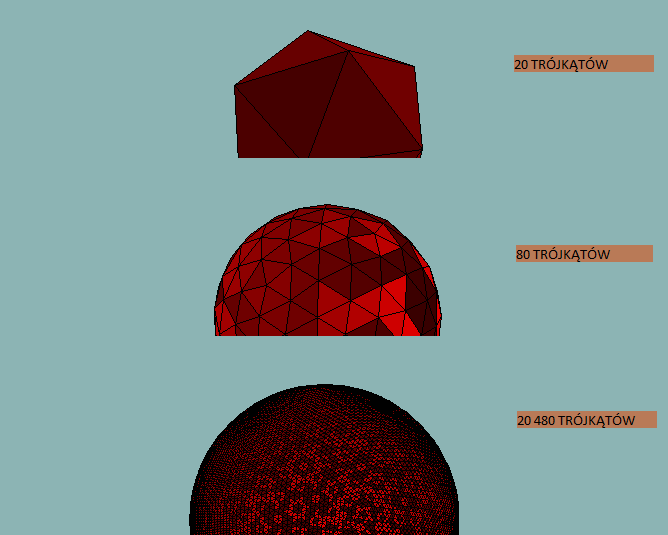
\includegraphics[width=\textwidth,height=4.5in]{kula.png}
    \caption{Ewolucja kuli.}
    \label{fig:kula}
\end{figure}

\subsection{Rysowanie kuli}

Kula została na początku zobrazowana przy pomocy dwudziestościanu foremnego, później każdą ścianę rekurencyjnie dzieliłem na cztery mniejsze trójkąty równoboczne i w zależności ile razy każdą ścianę pociąłem tyle miałem wynikowych trójkątów w kuli. Niestety przy braku optymalizacji w moim projekcie przy pocięciu każdej ściany  dwudziestościanu pięciokrotnie (20*4*4*4*4*4 = 20480 trójkątów) mój nienajgorszy sprzęt już ledwo dawał radę i renderował jedną klatkę na sekundę. Do testów zostawiłem trzykrotne cięcie ścian (20*4*4*4 = 1280 trójkątów) co daje i tak całkiem niezły efekt wizualny. Jak można zauważyć na załączonym obrazku na tym etapie trójkąty źle się jeszcze kolorowały, było to spowodowane wektorem w który zwórcone były ściany, na późnijeszym etapie udało się to poprawić, jednak wymagało to trochę szukania. 

\subsection{Implementacja algorytmu}

Został zaimplementowany model oświetlenia Phonga, którego parametrami w programie można sterować przy pomocy klawiszy F1-F6. Dodatkowo zostały dołożone klawisze F7-F12 do zmiany koloru wszystkich obiektów na scenie. Nie miałem żadnych problemów z implementacją tego modelu, przy każdej iteracji zamiast dawać stały zdefiniowany kolor obiektom po prostu zmieniam ich kolor w zależności od wekrota źródła światła do wektora wieloboku. Daje to całkiem dobry efekt wizualny i w przybliżeniu odzwierciedla warunki panujące w świecie rzeczywistym.

\section{Zgodność z założeniami}

Projekt z mojego punku widzenia spełnia założenia jakie były mu postawione. Samo oświetlenie musiałoby jednak zostać jeszcze wsparte cieniowaniem wieloboków, wtedy wyglądałoby kilkukrotnie bardziej realistycznie niż bez niego.

\section{Wnioski}

Model oświetlenia Phonaga nie odzwierciedla w pełni warunków rzeczywistych, ale jest bardzo prosty i nadaje się do implementacji nawet bardziej poważnych projektów graficznych. Do lepszego efektu brakuje jeszcze algorytmu cieniowania wieloboków. W ostatnim projekcie najwięcej problemów sprawiło mi narysowanie kuli, co na początku wydawało mi się prostym zadaniem. Sama implementacja modelu Phonga była tylko formalnością.

\end{document}